% Created by tikzDevice version 0.12 on 2019-06-13 13:14:36
% !TEX encoding = UTF-8 Unicode
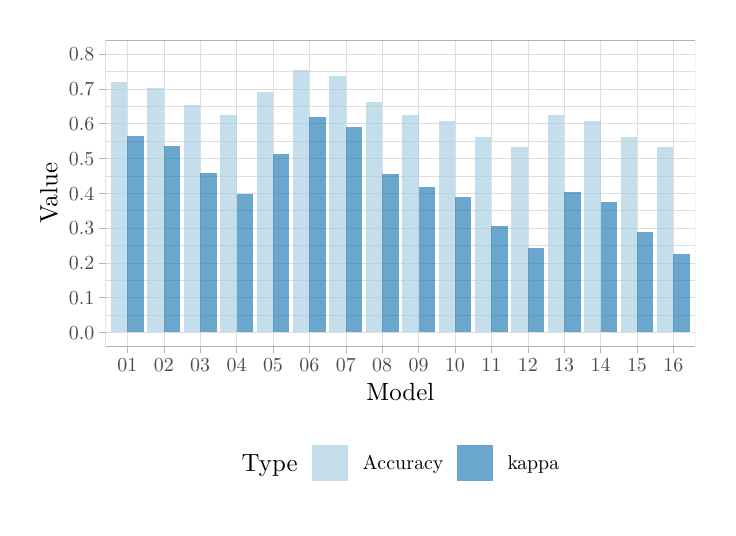
\begin{tikzpicture}[x=1pt,y=1pt]
\definecolor{fillColor}{RGB}{255,255,255}
\path[use as bounding box,fill=fillColor,fill opacity=0.00] (0,0) rectangle (245.72,173.45);
\begin{scope}
\path[clip] (  0.00,  0.00) rectangle (245.72,173.45);
\definecolor{drawColor}{RGB}{255,255,255}
\definecolor{fillColor}{RGB}{255,255,255}

\path[draw=drawColor,line width= 0.5pt,line join=round,line cap=round,fill=fillColor] (  0.00,  0.00) rectangle (245.72,173.45);
\end{scope}
\begin{scope}
\path[clip] ( 28.14, 58.30) rectangle (241.22,168.95);
\definecolor{fillColor}{RGB}{255,255,255}

\path[fill=fillColor] ( 28.14, 58.30) rectangle (241.22,168.95);
\definecolor{drawColor}{gray}{0.87}

\path[draw=drawColor,line width= 0.1pt,line join=round] ( 28.14, 69.62) --
	(241.22, 69.62);

\path[draw=drawColor,line width= 0.1pt,line join=round] ( 28.14, 82.19) --
	(241.22, 82.19);

\path[draw=drawColor,line width= 0.1pt,line join=round] ( 28.14, 94.76) --
	(241.22, 94.76);

\path[draw=drawColor,line width= 0.1pt,line join=round] ( 28.14,107.34) --
	(241.22,107.34);

\path[draw=drawColor,line width= 0.1pt,line join=round] ( 28.14,119.91) --
	(241.22,119.91);

\path[draw=drawColor,line width= 0.1pt,line join=round] ( 28.14,132.48) --
	(241.22,132.48);

\path[draw=drawColor,line width= 0.1pt,line join=round] ( 28.14,145.06) --
	(241.22,145.06);

\path[draw=drawColor,line width= 0.1pt,line join=round] ( 28.14,157.63) --
	(241.22,157.63);

\path[draw=drawColor,line width= 0.2pt,line join=round] ( 28.14, 63.33) --
	(241.22, 63.33);

\path[draw=drawColor,line width= 0.2pt,line join=round] ( 28.14, 75.90) --
	(241.22, 75.90);

\path[draw=drawColor,line width= 0.2pt,line join=round] ( 28.14, 88.48) --
	(241.22, 88.48);

\path[draw=drawColor,line width= 0.2pt,line join=round] ( 28.14,101.05) --
	(241.22,101.05);

\path[draw=drawColor,line width= 0.2pt,line join=round] ( 28.14,113.62) --
	(241.22,113.62);

\path[draw=drawColor,line width= 0.2pt,line join=round] ( 28.14,126.20) --
	(241.22,126.20);

\path[draw=drawColor,line width= 0.2pt,line join=round] ( 28.14,138.77) --
	(241.22,138.77);

\path[draw=drawColor,line width= 0.2pt,line join=round] ( 28.14,151.34) --
	(241.22,151.34);

\path[draw=drawColor,line width= 0.2pt,line join=round] ( 28.14,163.92) --
	(241.22,163.92);

\path[draw=drawColor,line width= 0.2pt,line join=round] ( 36.03, 58.30) --
	( 36.03,168.95);

\path[draw=drawColor,line width= 0.2pt,line join=round] ( 49.18, 58.30) --
	( 49.18,168.95);

\path[draw=drawColor,line width= 0.2pt,line join=round] ( 62.34, 58.30) --
	( 62.34,168.95);

\path[draw=drawColor,line width= 0.2pt,line join=round] ( 75.49, 58.30) --
	( 75.49,168.95);

\path[draw=drawColor,line width= 0.2pt,line join=round] ( 88.64, 58.30) --
	( 88.64,168.95);

\path[draw=drawColor,line width= 0.2pt,line join=round] (101.80, 58.30) --
	(101.80,168.95);

\path[draw=drawColor,line width= 0.2pt,line join=round] (114.95, 58.30) --
	(114.95,168.95);

\path[draw=drawColor,line width= 0.2pt,line join=round] (128.10, 58.30) --
	(128.10,168.95);

\path[draw=drawColor,line width= 0.2pt,line join=round] (141.26, 58.30) --
	(141.26,168.95);

\path[draw=drawColor,line width= 0.2pt,line join=round] (154.41, 58.30) --
	(154.41,168.95);

\path[draw=drawColor,line width= 0.2pt,line join=round] (167.56, 58.30) --
	(167.56,168.95);

\path[draw=drawColor,line width= 0.2pt,line join=round] (180.71, 58.30) --
	(180.71,168.95);

\path[draw=drawColor,line width= 0.2pt,line join=round] (193.87, 58.30) --
	(193.87,168.95);

\path[draw=drawColor,line width= 0.2pt,line join=round] (207.02, 58.30) --
	(207.02,168.95);

\path[draw=drawColor,line width= 0.2pt,line join=round] (220.17, 58.30) --
	(220.17,168.95);

\path[draw=drawColor,line width= 0.2pt,line join=round] (233.33, 58.30) --
	(233.33,168.95);
\definecolor{fillColor}{RGB}{31,120,180}

\path[fill=fillColor,fill opacity=0.66] ( 36.03, 63.33) rectangle ( 41.95,134.36);
\definecolor{fillColor}{RGB}{166,206,227}

\path[fill=fillColor,fill opacity=0.66] ( 30.11, 63.33) rectangle ( 36.03,153.77);
\definecolor{fillColor}{RGB}{31,120,180}

\path[fill=fillColor,fill opacity=0.66] ( 49.18, 63.33) rectangle ( 55.10,130.80);
\definecolor{fillColor}{RGB}{166,206,227}

\path[fill=fillColor,fill opacity=0.66] ( 43.27, 63.33) rectangle ( 49.18,151.57);
\definecolor{fillColor}{RGB}{31,120,180}

\path[fill=fillColor,fill opacity=0.66] ( 62.34, 63.33) rectangle ( 68.26,120.83);
\definecolor{fillColor}{RGB}{166,206,227}

\path[fill=fillColor,fill opacity=0.66] ( 56.42, 63.33) rectangle ( 62.34,145.68);
\definecolor{fillColor}{RGB}{31,120,180}

\path[fill=fillColor,fill opacity=0.66] ( 75.49, 63.33) rectangle ( 81.41,113.35);
\definecolor{fillColor}{RGB}{166,206,227}

\path[fill=fillColor,fill opacity=0.66] ( 69.57, 63.33) rectangle ( 75.49,142.01);
\definecolor{fillColor}{RGB}{31,120,180}

\path[fill=fillColor,fill opacity=0.66] ( 88.64, 63.33) rectangle ( 94.56,127.78);
\definecolor{fillColor}{RGB}{166,206,227}

\path[fill=fillColor,fill opacity=0.66] ( 82.72, 63.33) rectangle ( 88.64,150.09);
\definecolor{fillColor}{RGB}{31,120,180}

\path[fill=fillColor,fill opacity=0.66] (101.80, 63.33) rectangle (107.72,141.20);
\definecolor{fillColor}{RGB}{166,206,227}

\path[fill=fillColor,fill opacity=0.66] ( 95.88, 63.33) rectangle (101.80,158.18);
\definecolor{fillColor}{RGB}{31,120,180}

\path[fill=fillColor,fill opacity=0.66] (114.95, 63.33) rectangle (120.87,137.66);
\definecolor{fillColor}{RGB}{166,206,227}

\path[fill=fillColor,fill opacity=0.66] (109.03, 63.33) rectangle (114.95,155.98);
\definecolor{fillColor}{RGB}{31,120,180}

\path[fill=fillColor,fill opacity=0.66] (128.10, 63.33) rectangle (134.02,120.46);
\definecolor{fillColor}{RGB}{166,206,227}

\path[fill=fillColor,fill opacity=0.66] (122.18, 63.33) rectangle (128.10,146.42);
\definecolor{fillColor}{RGB}{31,120,180}

\path[fill=fillColor,fill opacity=0.66] (141.26, 63.33) rectangle (147.17,115.77);
\definecolor{fillColor}{RGB}{166,206,227}

\path[fill=fillColor,fill opacity=0.66] (135.34, 63.33) rectangle (141.26,142.01);
\definecolor{fillColor}{RGB}{31,120,180}

\path[fill=fillColor,fill opacity=0.66] (154.41, 63.33) rectangle (160.33,112.15);
\definecolor{fillColor}{RGB}{166,206,227}

\path[fill=fillColor,fill opacity=0.66] (148.49, 63.33) rectangle (154.41,139.80);
\definecolor{fillColor}{RGB}{31,120,180}

\path[fill=fillColor,fill opacity=0.66] (167.56, 63.33) rectangle (173.48,101.90);
\definecolor{fillColor}{RGB}{166,206,227}

\path[fill=fillColor,fill opacity=0.66] (161.64, 63.33) rectangle (167.56,133.92);
\definecolor{fillColor}{RGB}{31,120,180}

\path[fill=fillColor,fill opacity=0.66] (180.71, 63.33) rectangle (186.63, 93.95);
\definecolor{fillColor}{RGB}{166,206,227}

\path[fill=fillColor,fill opacity=0.66] (174.80, 63.33) rectangle (180.71,130.24);
\definecolor{fillColor}{RGB}{31,120,180}

\path[fill=fillColor,fill opacity=0.66] (193.87, 63.33) rectangle (199.79,114.01);
\definecolor{fillColor}{RGB}{166,206,227}

\path[fill=fillColor,fill opacity=0.66] (187.95, 63.33) rectangle (193.87,142.01);
\definecolor{fillColor}{RGB}{31,120,180}

\path[fill=fillColor,fill opacity=0.66] (207.02, 63.33) rectangle (212.94,110.29);
\definecolor{fillColor}{RGB}{166,206,227}

\path[fill=fillColor,fill opacity=0.66] (201.10, 63.33) rectangle (207.02,139.80);
\definecolor{fillColor}{RGB}{31,120,180}

\path[fill=fillColor,fill opacity=0.66] (220.17, 63.33) rectangle (226.09, 99.78);
\definecolor{fillColor}{RGB}{166,206,227}

\path[fill=fillColor,fill opacity=0.66] (214.25, 63.33) rectangle (220.17,133.92);
\definecolor{fillColor}{RGB}{31,120,180}

\path[fill=fillColor,fill opacity=0.66] (233.33, 63.33) rectangle (239.25, 91.57);
\definecolor{fillColor}{RGB}{166,206,227}

\path[fill=fillColor,fill opacity=0.66] (227.41, 63.33) rectangle (233.33,130.24);
\definecolor{drawColor}{gray}{0.70}

\path[draw=drawColor,line width= 0.5pt,line join=round,line cap=round] ( 28.14, 58.30) rectangle (241.22,168.95);
\end{scope}
\begin{scope}
\path[clip] (  0.00,  0.00) rectangle (245.72,173.45);
\definecolor{drawColor}{gray}{0.30}

\node[text=drawColor,anchor=base east,inner sep=0pt, outer sep=0pt, scale=  0.72] at ( 24.09, 60.85) {0.0};

\node[text=drawColor,anchor=base east,inner sep=0pt, outer sep=0pt, scale=  0.72] at ( 24.09, 73.42) {0.1};

\node[text=drawColor,anchor=base east,inner sep=0pt, outer sep=0pt, scale=  0.72] at ( 24.09, 86.00) {0.2};

\node[text=drawColor,anchor=base east,inner sep=0pt, outer sep=0pt, scale=  0.72] at ( 24.09, 98.57) {0.3};

\node[text=drawColor,anchor=base east,inner sep=0pt, outer sep=0pt, scale=  0.72] at ( 24.09,111.14) {0.4};

\node[text=drawColor,anchor=base east,inner sep=0pt, outer sep=0pt, scale=  0.72] at ( 24.09,123.72) {0.5};

\node[text=drawColor,anchor=base east,inner sep=0pt, outer sep=0pt, scale=  0.72] at ( 24.09,136.29) {0.6};

\node[text=drawColor,anchor=base east,inner sep=0pt, outer sep=0pt, scale=  0.72] at ( 24.09,148.87) {0.7};

\node[text=drawColor,anchor=base east,inner sep=0pt, outer sep=0pt, scale=  0.72] at ( 24.09,161.44) {0.8};
\end{scope}
\begin{scope}
\path[clip] (  0.00,  0.00) rectangle (245.72,173.45);
\definecolor{drawColor}{gray}{0.70}

\path[draw=drawColor,line width= 0.2pt,line join=round] ( 25.89, 63.33) --
	( 28.14, 63.33);

\path[draw=drawColor,line width= 0.2pt,line join=round] ( 25.89, 75.90) --
	( 28.14, 75.90);

\path[draw=drawColor,line width= 0.2pt,line join=round] ( 25.89, 88.48) --
	( 28.14, 88.48);

\path[draw=drawColor,line width= 0.2pt,line join=round] ( 25.89,101.05) --
	( 28.14,101.05);

\path[draw=drawColor,line width= 0.2pt,line join=round] ( 25.89,113.62) --
	( 28.14,113.62);

\path[draw=drawColor,line width= 0.2pt,line join=round] ( 25.89,126.20) --
	( 28.14,126.20);

\path[draw=drawColor,line width= 0.2pt,line join=round] ( 25.89,138.77) --
	( 28.14,138.77);

\path[draw=drawColor,line width= 0.2pt,line join=round] ( 25.89,151.34) --
	( 28.14,151.34);

\path[draw=drawColor,line width= 0.2pt,line join=round] ( 25.89,163.92) --
	( 28.14,163.92);
\end{scope}
\begin{scope}
\path[clip] (  0.00,  0.00) rectangle (245.72,173.45);
\definecolor{drawColor}{gray}{0.70}

\path[draw=drawColor,line width= 0.2pt,line join=round] ( 36.03, 56.05) --
	( 36.03, 58.30);

\path[draw=drawColor,line width= 0.2pt,line join=round] ( 49.18, 56.05) --
	( 49.18, 58.30);

\path[draw=drawColor,line width= 0.2pt,line join=round] ( 62.34, 56.05) --
	( 62.34, 58.30);

\path[draw=drawColor,line width= 0.2pt,line join=round] ( 75.49, 56.05) --
	( 75.49, 58.30);

\path[draw=drawColor,line width= 0.2pt,line join=round] ( 88.64, 56.05) --
	( 88.64, 58.30);

\path[draw=drawColor,line width= 0.2pt,line join=round] (101.80, 56.05) --
	(101.80, 58.30);

\path[draw=drawColor,line width= 0.2pt,line join=round] (114.95, 56.05) --
	(114.95, 58.30);

\path[draw=drawColor,line width= 0.2pt,line join=round] (128.10, 56.05) --
	(128.10, 58.30);

\path[draw=drawColor,line width= 0.2pt,line join=round] (141.26, 56.05) --
	(141.26, 58.30);

\path[draw=drawColor,line width= 0.2pt,line join=round] (154.41, 56.05) --
	(154.41, 58.30);

\path[draw=drawColor,line width= 0.2pt,line join=round] (167.56, 56.05) --
	(167.56, 58.30);

\path[draw=drawColor,line width= 0.2pt,line join=round] (180.71, 56.05) --
	(180.71, 58.30);

\path[draw=drawColor,line width= 0.2pt,line join=round] (193.87, 56.05) --
	(193.87, 58.30);

\path[draw=drawColor,line width= 0.2pt,line join=round] (207.02, 56.05) --
	(207.02, 58.30);

\path[draw=drawColor,line width= 0.2pt,line join=round] (220.17, 56.05) --
	(220.17, 58.30);

\path[draw=drawColor,line width= 0.2pt,line join=round] (233.33, 56.05) --
	(233.33, 58.30);
\end{scope}
\begin{scope}
\path[clip] (  0.00,  0.00) rectangle (245.72,173.45);
\definecolor{drawColor}{gray}{0.30}

\node[text=drawColor,anchor=base,inner sep=0pt, outer sep=0pt, scale=  0.72] at ( 36.03, 49.29) {01};

\node[text=drawColor,anchor=base,inner sep=0pt, outer sep=0pt, scale=  0.72] at ( 49.18, 49.29) {02};

\node[text=drawColor,anchor=base,inner sep=0pt, outer sep=0pt, scale=  0.72] at ( 62.34, 49.29) {03};

\node[text=drawColor,anchor=base,inner sep=0pt, outer sep=0pt, scale=  0.72] at ( 75.49, 49.29) {04};

\node[text=drawColor,anchor=base,inner sep=0pt, outer sep=0pt, scale=  0.72] at ( 88.64, 49.29) {05};

\node[text=drawColor,anchor=base,inner sep=0pt, outer sep=0pt, scale=  0.72] at (101.80, 49.29) {06};

\node[text=drawColor,anchor=base,inner sep=0pt, outer sep=0pt, scale=  0.72] at (114.95, 49.29) {07};

\node[text=drawColor,anchor=base,inner sep=0pt, outer sep=0pt, scale=  0.72] at (128.10, 49.29) {08};

\node[text=drawColor,anchor=base,inner sep=0pt, outer sep=0pt, scale=  0.72] at (141.26, 49.29) {09};

\node[text=drawColor,anchor=base,inner sep=0pt, outer sep=0pt, scale=  0.72] at (154.41, 49.29) {10};

\node[text=drawColor,anchor=base,inner sep=0pt, outer sep=0pt, scale=  0.72] at (167.56, 49.29) {11};

\node[text=drawColor,anchor=base,inner sep=0pt, outer sep=0pt, scale=  0.72] at (180.71, 49.29) {12};

\node[text=drawColor,anchor=base,inner sep=0pt, outer sep=0pt, scale=  0.72] at (193.87, 49.29) {13};

\node[text=drawColor,anchor=base,inner sep=0pt, outer sep=0pt, scale=  0.72] at (207.02, 49.29) {14};

\node[text=drawColor,anchor=base,inner sep=0pt, outer sep=0pt, scale=  0.72] at (220.17, 49.29) {15};

\node[text=drawColor,anchor=base,inner sep=0pt, outer sep=0pt, scale=  0.72] at (233.33, 49.29) {16};
\end{scope}
\begin{scope}
\path[clip] (  0.00,  0.00) rectangle (245.72,173.45);
\definecolor{drawColor}{RGB}{0,0,0}

\node[text=drawColor,anchor=base,inner sep=0pt, outer sep=0pt, scale=  0.90] at (134.68, 38.90) {Model};
\end{scope}
\begin{scope}
\path[clip] (  0.00,  0.00) rectangle (245.72,173.45);
\definecolor{drawColor}{RGB}{0,0,0}

\node[text=drawColor,rotate= 90.00,anchor=base,inner sep=0pt, outer sep=0pt, scale=  0.90] at ( 10.70,113.62) {Value};
\end{scope}
\begin{scope}
\path[clip] (  0.00,  0.00) rectangle (245.72,173.45);
\definecolor{fillColor}{RGB}{255,255,255}

\path[fill=fillColor] ( 72.80,  4.50) rectangle (196.56, 27.95);
\end{scope}
\begin{scope}
\path[clip] (  0.00,  0.00) rectangle (245.72,173.45);
\definecolor{drawColor}{RGB}{0,0,0}

\node[text=drawColor,anchor=base west,inner sep=0pt, outer sep=0pt, scale=  0.90] at ( 77.30, 13.13) {Type};
\end{scope}
\begin{scope}
\path[clip] (  0.00,  0.00) rectangle (245.72,173.45);
\definecolor{fillColor}{RGB}{255,255,255}

\path[fill=fillColor] (102.04,  9.00) rectangle (116.50, 23.45);
\end{scope}
\begin{scope}
\path[clip] (  0.00,  0.00) rectangle (245.72,173.45);
\definecolor{fillColor}{RGB}{166,206,227}

\path[fill=fillColor,fill opacity=0.66] (102.75,  9.71) rectangle (115.79, 22.74);
\end{scope}
\begin{scope}
\path[clip] (  0.00,  0.00) rectangle (245.72,173.45);
\definecolor{fillColor}{RGB}{255,255,255}

\path[fill=fillColor] (154.51,  9.00) rectangle (168.96, 23.45);
\end{scope}
\begin{scope}
\path[clip] (  0.00,  0.00) rectangle (245.72,173.45);
\definecolor{fillColor}{RGB}{31,120,180}

\path[fill=fillColor,fill opacity=0.66] (155.22,  9.71) rectangle (168.25, 22.74);
\end{scope}
\begin{scope}
\path[clip] (  0.00,  0.00) rectangle (245.72,173.45);
\definecolor{drawColor}{RGB}{0,0,0}

\node[text=drawColor,anchor=base west,inner sep=0pt, outer sep=0pt, scale=  0.72] at (121.00, 13.75) {Accuracy};
\end{scope}
\begin{scope}
\path[clip] (  0.00,  0.00) rectangle (245.72,173.45);
\definecolor{drawColor}{RGB}{0,0,0}

\node[text=drawColor,anchor=base west,inner sep=0pt, outer sep=0pt, scale=  0.72] at (173.46, 13.75) {kappa};
\end{scope}
\end{tikzpicture}
